\documentclass[a4paper,8pt, twocolumn]{extarticle}
\usepackage[utf8]{inputenc}
\usepackage{graphicx}
\usepackage{tikz}
\usetikzlibrary{arrows,shapes,positioning,snakes}
\usepackage[center]{caption}
\usepackage[english]{babel}
\usepackage[top=2.5cm, bottom=2.5cm, left=2.5cm, right=2.5cm]{geometry}

%---------------------------------------------
% Font packages
%---------------------------------------------
% \usepackage{lmodern}
% \usepackage{concmath}
% \usepackage{cmbright}
% \usepackage{kpfonts}
% \usepackage[adobe-utopia]{mathdesign}
\usepackage{fouriernc}
\usepackage[T1]{fontenc}

%---------------------------------------------
% Tabular package 
%---------------------------------------------
\usepackage{booktabs}
\usepackage{pifont}
\newcommand*\rot{\rotatebox{90}}
\newcommand*\rotsix{\rotatebox{60}}
\newcommand*\OK{\ding{51}}
\usepackage{multirow}
\usepackage{subfig}

%---------------------------------------------
% Math environment packages & command
%---------------------------------------------
\usepackage{amsmath}
\usepackage{amssymb}
\usepackage{array}
% \usepackage{mathrsfs}
\usepackage{array}
% \def\sgn{\mathop{\rm sgn}\nolimits} 
% \usepackage{bbm}


%---------------------------------------------
% item option
%---------------------------------------------
\usepackage{enumitem}
%\setitemize{itemsep=0pt}
\renewcommand{\labelitemi}{-}
%\renewcommand{\itemsep}{2em}

%---------------------------------------------
%HEADER & FOOTER
%---------------------------------------------
\usepackage{fancyhdr}
\pagestyle{fancy}

\renewcommand{\headrulewidth}{.15pt}
\fancyhead[C]{{\textsc{Micro Management in RTS Games}}} 
\fancyhead[L]{Page \thepage \ of \pageref{LastPage}}
\fancyhead[R]{DD2438}

\renewcommand{\footrulewidth}{.15pt}
\fancyfoot[C]{\thepage} 
% \fancyfoot[L]{truc}
% \fancyfoot[R]{bidule}

\usepackage{lastpage}

%---------------------------------------------
% two column option
%---------------------------------------------
\setlength{\columnsep}{0.7cm}


%---------------------------------------------
% Table of content
%---------------------------------------------
\usepackage[colorlinks,linkcolor=black, citecolor=black]{hyperref}

%---------------------------------------------
% Opening
%---------------------------------------------
\title{Artificial Intelligence \& Multi Agent Systems :\\ \textsc{Micro Management in Real Time Strategy Games}}
%\author{Björn \textsc{Holm}, Kilian \textsc{Demeulemeester} \\ \texttt{\{bjh,kiliande\}@kth.se}}
\author{Björn \textsc{Holm} \\ KTH \\ \texttt{bjh@kth.se}
    \and
Kilian \textsc{Demeulemeester} \\ KTH \\ \texttt{kiliande@kth.se}}
\date{\today}

%---------------------------------------------
% Numerotation Handling
%---------------------------------------------
 %\setcounter{section}{3}
 \usepackage[explicit]{titlesec}
  %\titleformat{<command>}[<shape>]{<format>}{<label>}{<sep>}{<before>}[<after>]
	\titleformat{\section}[block]{\normalsize\bfseries\filcenter}{\Roman{section}.}{1em}{#1}
	\titleformat{\subsection}[block]{\normalsize\bfseries}{\emph{\Alph{subsection}.}}{1em}{\emph{#1}}
 %\titleformat{\section}[hang]{\normalfont\Large\bfseries}%
     %{}{8pt}%
     %{\arabic{section}. #1}


%---------------------------------------------
% Dummy text
%---------------------------------------------
\usepackage{lipsum}

%---------------------------------------------
% Bibliography package
%---------------------------------------------
\usepackage{url}
\hypersetup{urlcolor=black}
\usepackage{breakurl}

%---------------------------------------------
% Item package option 
%---------------------------------------------
\newenvironment{shortitem}{
    \begin{itemize}
        \setlength{\topsep}{1ex}
        \setlength{\partopsep}{1ex}
        \setlength{\itemsep}{0ex}
        \setlength{\parskip}{0pt}
        \setlength{\parsep}{1ex}
    }{\end{itemize}}

\newenvironment{enum}{
    \begin{enumerate}
        \setlength{\topsep}{1ex}
        \setlength{\partopsep}{1ex}
        \setlength{\itemsep}{0ex}
        \setlength{\parskip}{0pt}
        \setlength{\parsep}{1ex}
    }{\end{enumerate}}
    

\newenvironment{descri}{
    \begin{description}
        \setlength{\topsep}{1ex}
        \setlength{\partopsep}{1ex}
        \setlength{\itemsep}{0ex}
        \setlength{\parskip}{0pt}
        \setlength{\parsep}{1ex}
    }{\end{description}}

%---------------------------------------------
% Algorithm form
%---------------------------------------------
    \usepackage{amsthm}
    \usepackage{thmtools}
    \declaretheorem[thmbox=M]{algorithm}
%\newtheorem{algorithm}{Algorithm}[section]
\newtheorem{criteria}{Criteria}[section]
\newtheorem{problem}{Problem}
\newtheorem{subproblem}{Problem}[section]
\newtheorem{definition}{Definition}[section]

\begin{document}

% % Indentation size
% \setlength\parindent{0em}
% 
% \setlength{\itemsep}{0pt}

\maketitle

\begin{bfseries} Abstract -- \end{bfseries}
\emph{
Real Time Strategy games (RTS) present a complete simulated environment that pose many interesting challenges to the research of Artificial Intelligence (AI).
Among these challenges are the huge branching factor of play and constrained time for decision.
In this paper we restrict ourselves the management of military troops at a micro-level, that is: given a scenario with for example 10 vs.\ 10 units that have already discovered each other, which actions should our units perform?
}

\emph{
We describe three different approaches: using scripted behaviors, Alpha-Beta search and UCT search, for unit control in combat scenarios in the game Stacraft: Broodwar, using the Broodwar API (BWAPI) for interfacing with the game \cite{BWAPI}.
}


\vspace{0.5cm}
\hrule

%\tableofcontents

\section{Introduction and Background}
RTS games provide a very interesting platform for developing and testing multi agent coordination.
%In game theoretic terms, RTS games can be considered symmetric, non-zero-sum, simultaneous, imperfect information, combinatorial games.
That which separates RTS games the most from traditional games like chess is the huge branching factor when taking every possible combination of every unit's allowed moves into account, and even in a 10 vs 10 unit battle, all the different ways a battle could play out quickly grows beyond what is feasible to perform an exhaustive search on.
On top of that, a complete model of how the game mechanics work might not be available, and new decisions have to be taken in only the time between each frame
\footnote{
As an example, in the 2011 AIIDE \textsc{Starcraft} AI Competition, 55 ms were given to the bots per frame.
\url{https://skatgame.net/mburo/sc2011/rules.html}
}
.

The game of \textsc{Starcraft} is a good platform for evaluating different methods for addressing these difficulties and several tournaments are held yearly
\footnote{
\url{http://www.sscaitournament.com/}\\ 
\url{http://www.aiide.org/starcraft} \\
\url{http://bots-stats.krasi0.com/} (ladder)
}
.

The game can be roughly divided into two parts, managing the economy (to produce combat units), and managing combat units.
The term \emph{micromanagement} can be used to describe the low-level actions performed by the player in both the economic and the combat aspects of the game, but we will henceforth only refer to it in the context of combat.
For micromanagement, most of current bots such as \emph{UAlbertaBot} and \emph{Skynet}, the two top winning bots in the 2013 AIIDE \textsc{Starcraft} AI competition,
\footnote{\url{http://webdocs.cs.ualberta.ca/~cdavid/starcraftaicomp/report2013.shtml}
}
use scripted behaviors.
Scripted behaviors are usually relatively simple preprogrammed descriptions of what course of action should be taken for a given state of the world, for example, attack the closest enemy.
These algorithms provide good results in term of computational speed but often lack in foresight.
Another approach is to use search-based methods, which naturally adapt to the current situation.
Looking ahead often allows for finding winning variations where scripted solutions fail because they cannot be preprogrammed to handle every possible state that is in theory winnable.
For reference, in the games of Chess or Go, the problem of finding an optimal winning solution has been proven to be NP-HARD \cite{nphard}.

%\section{Related Work}
%...

However even classical search based method have to be modified in order to take in account simultaneous and non-instantaneous moves of RTS games.
In \cite{abcd} a fast search method -- Alpha-Beta search for durative moves -- is presented and proven better than commonly used AI scripts (with battle up to 8 vs 8 units). 
\cite{wargusuct} investigates the use of UCT -- a Monte-Carlo planning algorithm for this problem -- and provide a battle planning strategy better than several baselines and even a human player.


\section{Problem statement}
In this paper we only focus of the \textbf{\textit{micromanagement of the units of two players engaging in combat in RTS games}}.
Each player is given a number of units, the whole map is visible and the goal is to control these units so as to kill all enemy units while minimizing the losses on the own team.

The main challenging questions are:
\begin{enumerate}
        \setlength{\topsep}{0pt}
        \setlength{\partopsep}{0pt}
        \setlength{\itemsep}{0pt}
        \setlength{\parskip}{0pt}
        \setlength{\parsep}{0pt}
    \item Where to move the units?
    \item Which enemies to attack?
    \item How to coordinate well with team members?
    \item How to detect and exploit opponent weaknesses?
\end{enumerate}


\section{Approaches to micromanagement}
There are at least two different groups of algorithms for solving micromanagement: scripted and searching.
In scripted behaviors the action to be taken for a given state is determined by some predefined rules, and for example encoded in a finite-state machine or behavior tree.
This is perhaps the most widely used technique today, the built-in AI of \textsc{Starcraft} seems to use some variant of it.
Searching algorithms on the other hand work by simulating the game into the future, trying out different move combinations and counter move combinations as far into the future as there is time to simulate, and choosing the most promising course of action.

\subsection{Scripted behaviors}
The three scripted behaviors we have implemented are
\begin{shortitem}
\item \texttt{Attack Closest:}					Every unit attacks their closest enemy.
\item \texttt{Attack Closest -- No Overkill:}	Every unit attacks their closest enemy that is not already attributed enough damage to kill it soon.
\item \texttt{Kiting:}							Every unit attacks their closest enemy while applying a kiting strategy, more on this later.
\end{shortitem}

Note that out of these, only in the \texttt{Attack Closest -- No Overkill} do the units share any information with each other, namely which target they attack next; in the other two scripts every unit acts on its own.

\subsection {Searching algorithms}
The two searching algorithms we have implemented are
\begin{shortitem}
\item \texttt{UCT-Searching:}	UCT, Upper Confidence bounds for Trees, a Monte-Carlo Tree Search algorithm.
\item \texttt{ABCD-Searching:}	ABCD, Alpha-Beta Considering Durations, a searching algorithm based on the alpha-beta algorithm adapted to durative moves in \cite{abcd}.
\end{shortitem}
In these algorithms, the units not only share information but are rather considered as a single entity, like the fingers of a hand, and are coordinated.
More on these later.


\section{Kiting}
\label{kiting}

Kiting behavior is worth more explanation. 
We based our algorithm on the work of \cite{kiting}. 

\begin{definition}[Kiting]
    Kiting (to kite) is to move units around to make the enemy chase them and thus not be able to attack as much, or not at all. 
    Kiting can be summarize as:
    \begin{shortitem}
    \item Move out of range
    \item Turn back and shoot at the enemy
    \item Repeat
    \end{shortitem}
\end{definition}

The behavior tree used by the units achieving \texttt{Kiting} is depicted in Figure \ref{behaAttackClos}.

\begin{figure}[h!t]
\centering
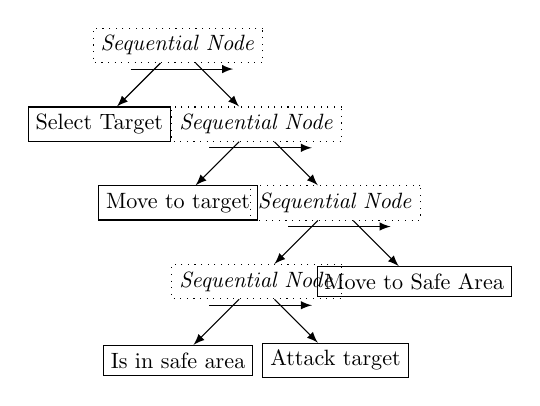
\begin{tikzpicture}[node distance = 1 cm]
    \tikzstyle{leaf}=[rectangle, align=center, scale=0.8, draw]
    \tikzstyle{node}=[rectangle,dotted, align=center, scale=0.8, draw]
    \tikzstyle{tt}=[rectangle,scale=0.8, align=center]
    \tikzstyle{link}=[->,thin,>=latex]
    \node[node] (start) at (1,4) {\emph{Sequential Node}};
    \node[tt] (start1) at (0.3,3.7) {};
    \node[tt] (end1) at (1.8,3.7) {};
    \draw[link] (start1)--(end1);

    \node[leaf] (target) at (0,3) {Select Target};

    \node[node] (seqNode) at (2,3) {\emph{Sequential Node}};
    \node[tt] (start2) at (1.3,2.7) {};
    \node[tt] (end2) at (2.8,2.7) {};
    \draw[link] (start2)--(end2);

    \node[leaf] (leafMove) at (1,2) {Move to target};
    \node[node] (seqAttack) at (3,2) {\emph{Sequential Node}};
    \node[tt] (start3) at (2.3,1.7) {};
    \node[tt] (end3) at (3.8,1.7) {};
    \draw[link] (start3)--(end3);

    \node[node] (attackNode) at (2,1) {\emph{Sequential Node}};
    \node[tt] (start4) at (1.3,0.7) {};
    \node[tt] (end4) at (2.8,0.7) {};
    \draw[link] (start4)--(end4);

    \node[leaf] (moveSafe) at (4,1) {Move to Safe Area};

    \node[leaf] (isSafe) at (1,0) {Is in safe area};
    \node[leaf] (attack) at (3,0) {Attack target};

    \draw[link] (start)--(target);
    \draw[link] (start)--(seqNode);

    \draw[link] (seqNode)--(leafMove);
    \draw[link] (seqNode)--(seqAttack);

    \draw[link] (seqAttack)--(attackNode);
    \draw[link] (seqAttack)--(moveSafe);

    \draw[link] (attackNode)--(attack);
    \draw[link] (attackNode)--(isSafe);
\end{tikzpicture}
\caption{Behavior tree for kiting}
\label{behaAttackClos}
\end{figure}

When selecting the target our bot try to select a target on which a kiting strategy can be used (for instance unit \texttt{A} can not kite another unit \texttt{A}). 
If it can not find any kitable unit then a classic attack is perform (\emph{fight to the death while standing on your position}).

As in paper \cite{kiting} the kiting bot uses an influence map for performing kiting: a 2D matrix $I_{enemy}$.

Let $e$ be an enemy. $e$ has an influence of the area $(i,j)$ of the map if the area can be reached by the enemy before performing kiting.
This relation is denoted $e \textasciitilde (i,j)$.

\begin{multline*}
    e \textasciitilde (i,j) \Leftrightarrow \\ d(e,(i,j)) \leq e.attackRange + e.speed * kitingTime
\end{multline*}

Then the influence matrix is define as:
$$
I_{enemy}(i,j) = \sum_{e \textasciitilde (i,j)}e.DPF \text{ where } DPF = \frac{e.damage}{e.cooldown}  
$$

(DPF is the damage per frame --  average damage of an unit.)

Using this matrix each unit can compute its closest safe position.
Then an attack is performed each time the unit is in a safe area.
Figure \ref{influenceMatrix} shows the influence matrix of a group of 3 units.

\begin{center}
    \begin{figure}[h!t]
        \centering
        \includegraphics[width=0.4\columnwidth]{fig/InfluenceMap.ps}
        \caption{Influence matrix created by a group of 3 units \\ 
        Darker grey means bigger threat}
        \label{influenceMatrix}
    \end{figure}
\end{center}



\section{Game Combat Model}

\subsection{Modeling}
To be able to search over possible future states of the game it is necessary to be able to represent such future states,
and since is not possible to try the outcomes of different actions through the \textsc{Starcraft} engine, 
we must create a model of the game and simulate this separately.
A similar model is presented in \cite{portfolio} but the one presented here allows for more detailed reproductions of all of the timings and various intricacies of the game engine, possibly at the expense of computation time.
It also allows for modeling things such as splash damage and spells, but does not, at the moment, consider unit collisions.

In order to search for a solution, we created the following components:

\begin{descri}
%STATE
\item[State] $s=<t,U_p,U_e,E,S_A>$:
\begin{shortitem}
\item Current game time $t$
\item Set $U_p$ of the player's units
\item Set $U_e$ of the enemy's units
\item Set of pending effects $E$
\item Set $S_A$ of allowed sets of actions that can be performed from $s$ (multiple units may be be ordered to at the same time)
\end{shortitem}

%UNIT
\item[Unit] $u = <p,hp,b_a,b_m,S_A>$
\begin{shortitem}
\item Position $p = (x,y) \in \mathbb{Z}^2$
\item Current hit points $hp$ ($\Leftrightarrow$ health points)
\item Booleans indicating if the unit can attack $b_a$ or move $b_m$
\item A static set $S_A$ of all possible actions that the unit can perform
\end{shortitem}

There are many different actions, such as: attack, move, deploy, spells, etc.
%ACTION
\item[Action] $a=<pc,E>$
\begin{shortitem}
\item Precondition $pc$ for the action to be allowed in the current gamestate
\item Set $E$ of effects the action will have on the gamestate.
	Most effects are delayed and will not alter the gamestate right away, and will instead be put in the state's set of pending effects $E$.
\end{shortitem}

Effects, in turn, can have various parameters, such as \emph{attacker} and \emph{target} in the case of an attack effect, or \emph{unit} and \emph{direction} in the case of an move effect.
The only things they have in common is that they have an frame offset $t_e$ and that they may modify any part of the gamestate when applied.
%EFFECT
\item[Effect] $e=<t_e>$
\begin{shortitem}
\item Frame offset $t_e$ relative to the frame on which the action it is part of was issued. At this offset the effect is to be applied to the gamestate
\end{shortitem}
\end{descri}

Table \ref{effectUnits} presents the effect corresponding to an attack for two kinds of units (a \texttt{Marine} and a \texttt{Firebat}).
As we can see units' actions have impacts on \emph{future} frames.

\begin{table}[h!t]
    \centering
\subfloat{
\centering
\begin{tabular}{cc|ccc}
&& unit can & Decrease & Weapon in \\
&& not move & $target.hp$ & cooldown \\
\hline
\multirow{4}{*}{\rot{Frame}} 
& 0    & \OK &     & \OK  \\
& 1    & \OK & \OK & \OK  \\
& 2-5  & \OK &     & \OK  \\
& 6-17 &     &     & \OK  \\
\end{tabular}
}
\\
\subfloat{
\centering
\begin{tabular}{cc|ccc}
&& unit can & Decrease & Weapon in \\
&& not move & $target.hp$ & cooldown \\
\hline
\multirow{4}{*}{\rot{Frame}} 
& 0-4   & \OK &     & \OK  \\
& 5-6   & \OK & \OK & \OK  \\
& 7-10  & \OK &     & \OK  \\
& 11-24 &     &     & \OK  \\
\end{tabular}
}
\caption{Example of effects $e=<u,target,t_e,type>$}
\label{effectUnits}
\end{table}

\subsection{State generation}

Algorithm \ref{algGeneration} explains how a new state is constructed, taking into account the actions performed to go from the parent to the new child and the pending effects.

\begin{figure}[h!t]
\begin{algorithm}[State generation]
%\begin{descri} 
The following algorithm describes how a new state $s_1=<t,U_p,U_e,E,S_A>$ is constructed from its parent $s_0$ and a set of allowed actions $a$. \ \\
%\end{descri}

\textbf{Function} $descend(s_0,A)$:
\begin{enum}
\item $s_1.t = s_0.t$
\item $s_1.U_p = s_0.U_p$
\item $s_1.U_e = s_0.U_e$
\item $s_1.E = s_0.E \cup A.E$
\item Create the set $s_1.S_A$ of allowed sets of actions available from $s_1$

\item \textbf{While} $S_A$ is empty and no team has won
\begin{enum}
	\item $s_1.t = s_1.t + 1$
	\item apply all effects $\{e \in s_0.E | e.t_e = s_1.t\}$ to $s_1$
	\item $s_1.E = \{e \in s_0.E | e.t_e > s_1.t\}$
	\item Create the set $s_1.S_A$ of allowed sets of actions available from $s_1$
\end{enum}

\item \textbf{Return} $s_1$

\end{enum}
\label{algGeneration}
\end{algorithm}
\end{figure}



\subsection{Allowed actions generation}
The allowed actions for each game state corresponds to which the children of each node are in the game tree.
The problem is only that in RTS games, the number of all allowed actions quickly grows beyond what is feasible to perform an exhaustive search on.
Consider that even in as small an battle as that between 10 units, 5 on each team, each having 5 possible actions
(move \texttt{North}, move \texttt{South}, move \texttt{East}, move \texttt{West}, attack
lead to $5^10 = 9765625$ possible combinations of orders only for the first frame.
\footnote{This number is then lower or even zero for subsequent frames while the units are busy executing their given orders, but may grow again when the units are finished.}
Which the allowed actions are for each state depends on the method being used, two possible such methods are:

\begin{shortitem}
\item \texttt{PlayerActionSubset:}
	Taking the huge number of allowed action combinations into account, one way of addressing this issue is to only consider a random subset of them.
\item \texttt{UnitAction:}
	Another way of managing the branches of the tree is to not generate complete combinations of one action for every unit at every level of the tree, but instead only considering the allowed actions of a single unit at each level in the tree.
	This way, it may be possible to prune bad choices for specific units more efficiently, but unless the unit is the one whose's actions are consider at the root of the tree, the same action may be evaluated again in other branches of the tree.
\end{shortitem}

Figure \ref{tree} displays an example of a tree constructed and traversed by the algorithm. Only some nodes of the tree are constructed.
As shown in Algorithm \ref{algGeneration}, a child's frame number is incremented until either a terminal state is reached or any actions become available.
As an example, assuming that our set of actions attributes an attack sequence to each of the \texttt{Marine} in the battleground and according to Table \ref{effectUnits}, there will not be any new actions available until the sixth frame.

\begin{figure}[h!t]
\centering
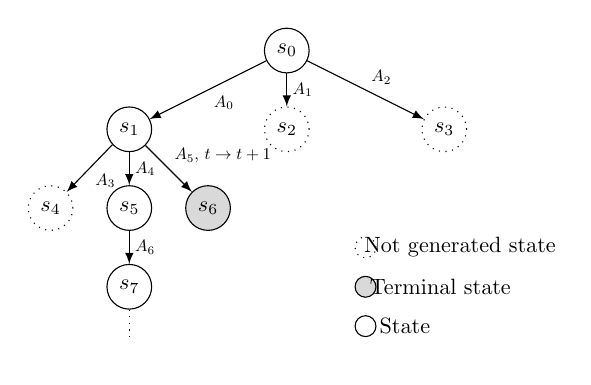
\begin{tikzpicture}[node distance = 1cm]
    \tikzstyle{node}=[circle,align=center,scale=0.8,draw]
    \tikzstyle{nodenotgen}=[circle,dotted,align=center,scale=0.8,draw]
    \tikzstyle{nodeterm}=[circle,fill=gray!30,align=center,scale=0.8,draw]
    \tikzstyle{link}=[->,thin,>=latex]
    
    \node[node] (s0) at (4,4) {$s_0$};

    \node[node] (s1) at (2,3) {$s_1$};
    \node[nodenotgen] (s2) at (4,3) {$s_2$};
    \node[nodenotgen] (s3) at (6,3) {$s_3$};

    \node[nodenotgen] (s4) at (1,2) {$s_4$};
    \node[node] (s5) at (2,2) {$s_5$};
    \node[nodeterm] (s6) at (3,2) {$s_6$};

    \node[node] (s7) at (2,1) {$s_7$};

    \node[auto,scale=0.8] (s8) at (2,0.2) {};
    
    \draw[link] (s0) to node [auto,scale=0.6] {$A_0$} (s1); 
    \draw[link] (s0) to node [auto,scale=0.6] {$A_1$} (s2);
    \draw[link] (s0) to node [auto,scale=0.6] {$A_2$} (s3);
    \draw[link] (s1) to node [auto,scale=0.6] {$A_3$} (s4);
    \draw[link] (s1) to node [auto,scale=0.6] {$A_4$} (s5);
    \draw[link] (s1) to node [auto,scale=0.6] {$A_5$, $t \rightarrow t+1$} (s6);
    \draw[link] (s5) to node [auto,scale=0.6] {$A_6$} (s7);
    \draw[-,>=latex,dotted] (s7) to (s8);
    

    %LEGEND

    \node[node] (l1) at (5,0.5) {}; % {$\phantom{s_1}$};
    \node[nodeterm] (l2) at (5,1)  {}; %{$\phantom{s_1}$};
    \node[nodenotgen] (l3) at (5,1.5) {}; %{$\phantom{s_1}$};
    \node[align=left,rectangle,scale=0.8] (l1t) at (5.5,0.5) {State};
    \node[align=left,rectangle,scale=0.8] (l2t) at (5.95,1.0) {Terminal state};
    \node[align=left,rectangle,scale=0.8] (l3t) at (6.2,1.5) {Not generated state};

\end{tikzpicture}
\caption{Example of a tree}
\label{tree}
\end{figure}



\subsection{Move ordering}
After selecting which are the allowed sets of actions from each state, that is, the children of each node in the game tree, it is of further interest to prune the less promising branches of the tree.
For this, move ordering, or deciding in which order to evaluate the children, is important since it allows for earlier pruning.
The time restriction of RTS games greatly limits the maximum number of children that can be explored, and it is well known that a good move ordering can greatly improve performance.

One interesting way of doing this is presented in \cite{portfolio}.
Their idea is to first consider the actions produced by some scripted behaviors that generally perform quite good.



\subsection{State evaluation}
For comparing how good states are, it is necessary to make use of some evaluation function.
The evaluation functions suggested by \cite{abcd} are the following:
\begin{shortitem}
\item Straight Forward Evaluations:
$$
    \displaystyle{SFE(s) = \sum_{u \in s.U_p} u.hp - \sum_{u \in s.U_e} u.hp } 
$$

\item Life Time Damage:
$$
    \displaystyle{LTD(s) = \sum_{u \in s.U_p} u.hp \cdot u.DPS- \sum_{u \in s.U_e} u.hp \cdot u.DPS } 
$$

\item Life Time Damage 2:
$$
    \displaystyle{LTD2(s) = \sum_{u \in s.U_p} \sqrt{u.hp} \cdot u.DPS - \sum_{u \in s.U_e} \sqrt{u.hp} \cdot u.DPS } 
$$

\item Playouts:
	Another way of evaluating the state commonly used in Monte Carlo Tree Search algorithms is playouts. In essence the game state is played out to a terminal state either by picking random moves for the players or by using some scripted behaviors.
\end{shortitem}


$SFE$ doesn't take into account units' damage per second, DPS -- which is an essential information during a battle. 
$LTD$ present a good estimation of DPS but does not favor equal hit point distribution among the units. 
Ultimately $LTD2$ measures the DPS and favor the greatest number of units remaining\footnote{Having two units with $50$ hit points means higher DPS than one with $100$ hit points.}.






\section{Search}
Both of the search algorithms we implemented perform a completely new search for solutions every game frame and no information is kept between frames.

\subsection{UCT Search}
UCT, or Upper Confidence bound for Trees, is the most popular Monte Carlo Tree Search algorithm for playing games that are otherwise hard for computers to handle. \cite{mcts}
This algorithm has recently seen success in the game of Go, but more relevant to our topic, also been applied to games such as Arimaa, and even RTS games.
Arimaa is interesting because it has an average branching factor of 17000, compared to chess, which only has 35. \cite{arimaawiki}
For a review of how UCT works we refer to \cite{mcts}.

\subsection{ABCD Search}
%move to related work?
In \cite{abcd}, an extended version of alpha-beta pruning, which is a well-known searching algorithm, was used for micromanagement. 
They were able to find good solutions for 8 v.s. 8 unit scenarios in 5 ms, achieving around a 80\% win rate against their best script.

In order to use alpha-beta algorithm it is necessary to separates the player's actions and its opponents action. We used the method \texttt{PlayerActionSubset} to do so. 

The children of a node are the restriction of its children to only one player set of actions:
$$
S_{A|p} = \{A \in S_A | \forall a \in A, a \text{ is an action performed by $p$}\}
$$
Algorithm \ref{algABCD} presents the ABCD algorithm.
The main distinction with the ``classic'' alpha-beta algorithm is that there is not a perfect alternation between $MAX$ and $MIN$. Once a state has no possible actions, we move in time until an action can be performed for one of the player. 
%Figure \ref{figABCD} shows an example of such a tree: once we've reached a state where no action can be made for both player, we advance in time. In this new frame, there is an action for $MAX$. Therefore it is still he who is considered as the current player.

\begin{figure}[h!t]
    \begin{algorithm}[ABCD (Alpha-Beta Considering Durations)]
Let $s_0$ be the root node, $MAX$ be the player and $MIN$ the opponent. The algorithm return the best move compute by $ABCD(s_0,d_{max},-\infty,+\infty,MAX)$ where: \ \\

        \textbf{Function} $ABCD(s,d,\alpha,\beta,p)$:
        \begin{enum}
        \item \textbf{If} ($s$ is a terminal state) \textbf{Return} $LTD2(s)$
        \item \textbf{Else}
            \begin{enum}
            \item If $S_{A|p} \neq \emptyset$ 

            \begin{enum}
            \item \textbf{While} $S_{A|p} \neq \emptyset$
                \begin{enum}
                \item Pop $s_1$ from $S_{A|p}$ 
                \item Let $v = ABCD(s_1,d-1,\alpha,\beta,\bar{p})$
                \item \textbf{If} $p = MAX$ and $(v > \alpha)$ \textbf{then} $\alpha = v$
                \item \textbf{If} $p = MIN$ and $(v < \beta)$ \textbf{then} $\beta= v$
                \item \textbf{If} $\alpha \geq \beta$ \textbf{then break} 
                \end{enum}
            \item \textbf{Return} $(p = MAX) ? \alpha : \beta$ 
            \end{enum}
        \item \textbf{Else if} $S_{A|\bar{p}} \neq \emptyset$
            \begin{enum}
            \item \textbf{Return} $ABCD(s,d,\alpha,\beta,\bar{p})$
            \end{enum}
        \item \textbf{Else} 
            \begin{enum}
            \item Advance in time to state $s'$ for which $S'_A \neq \emptyset$
            \item \textbf{Return} $ABCD(s',d,\alpha,\beta,p)$
            \end{enum}
        \end{enum}
        \end{enum}
        \ \\
        And $s$ being considered as a \textbf{terminal state} if $d_{max}$ is reached, the time is elapsed or the state is a winning/loosing situation.
        \label{algABCD}
    \end{algorithm}
\end{figure}



\section{Results}



%At the present time our micromanagement bots need more development (UCT search) and/or more testing. This part will be accomplished in a future work.

So far all of the testing has been made by testing our bots against the built-in AI of \textsc{Starcraft}. While not sure of how this AI work it seems to pack all unit together and send them in a suicide mission (move to closest target, attack it, repeat). 

This AI is able to defeat the \texttt{Attack Closest} bot on almost every game (10 vs 10 often leads to 3--4 man standing for the opponent team).
Indeed, \texttt{Attack Closest} do not present any cooperative work neither fleeing behavior for in danger units. However, \texttt{Attack Closest -- No Overkill} defeat the AI on almost every game with a ration of \textasciitilde25\% of player units still alive. This bot offers a very good cooperation between unit.

Since kiting behavior can not be tested with the same kind of units we tested it by fighting slow powerful but low range units (\texttt{zealot}) versus fast long range units (\texttt{Vulture}). 
In that situation our bot was able to defeat the opponent team almost every time (even in scenario such as 3 (us) VS 10 (opponent)). 
Theoretically, one unit should be enough. However the bot attack sequence sometimes gets stuck in attack mode (our bot was unable do detect that the attack has been performed) and therefore the \texttt{Vulture} unit is destroyed almost instantly by the \texttt{Zealots}.

Our implementation of searching algorithms (ABCD and UCT) do not success in defeating the built-in AI.
However, $\textasciitilde 20000$ nodes can be explored by those algorithm in a reasonable time ($\textasciitilde 50ms$). 


\vspace{0.5cm}
\hrule
\vspace{0.5cm}
\begin{bfseries} Conclusion -- \end{bfseries}
    \emph{While extremely complicated in term of searchability, RTS game are indeed a solid platform for developing and testing multi agent cooperative behaviors. Our work was focused on micro management and so far we were able to implement some ``classic behaviors'' (\emph{i.e} behaviors used by real human player).} 
    \emph{However, in a future work we want to develop the UCT search and accomplish statistical comparison of the bots. We also aim at improving the bots to fight with 3 kinds of units.} 



\nocite{*}
\bibliographystyle{plain}
\bibliography{bibliography}

\end{document}
